\subsection{W-DCGAN}
\label{sec:exp-w-dcgan}
We present the evolution of the Inception score and losses in Figures \ref{fig:exp-w-dcgan-is} and \ref{fig:exp-w-dcgan-losses}, respectively. We did not expect to a get good performance using this setup since we did not implement any method enforcing the Lipschitz continuity of the discriminator functions, which is required by WGAN. These results coincide with our expectations.
   
\begin{figure}[H]
    \centering
    \begin{subfigure}[t]{0.49\textwidth}
        \centering
		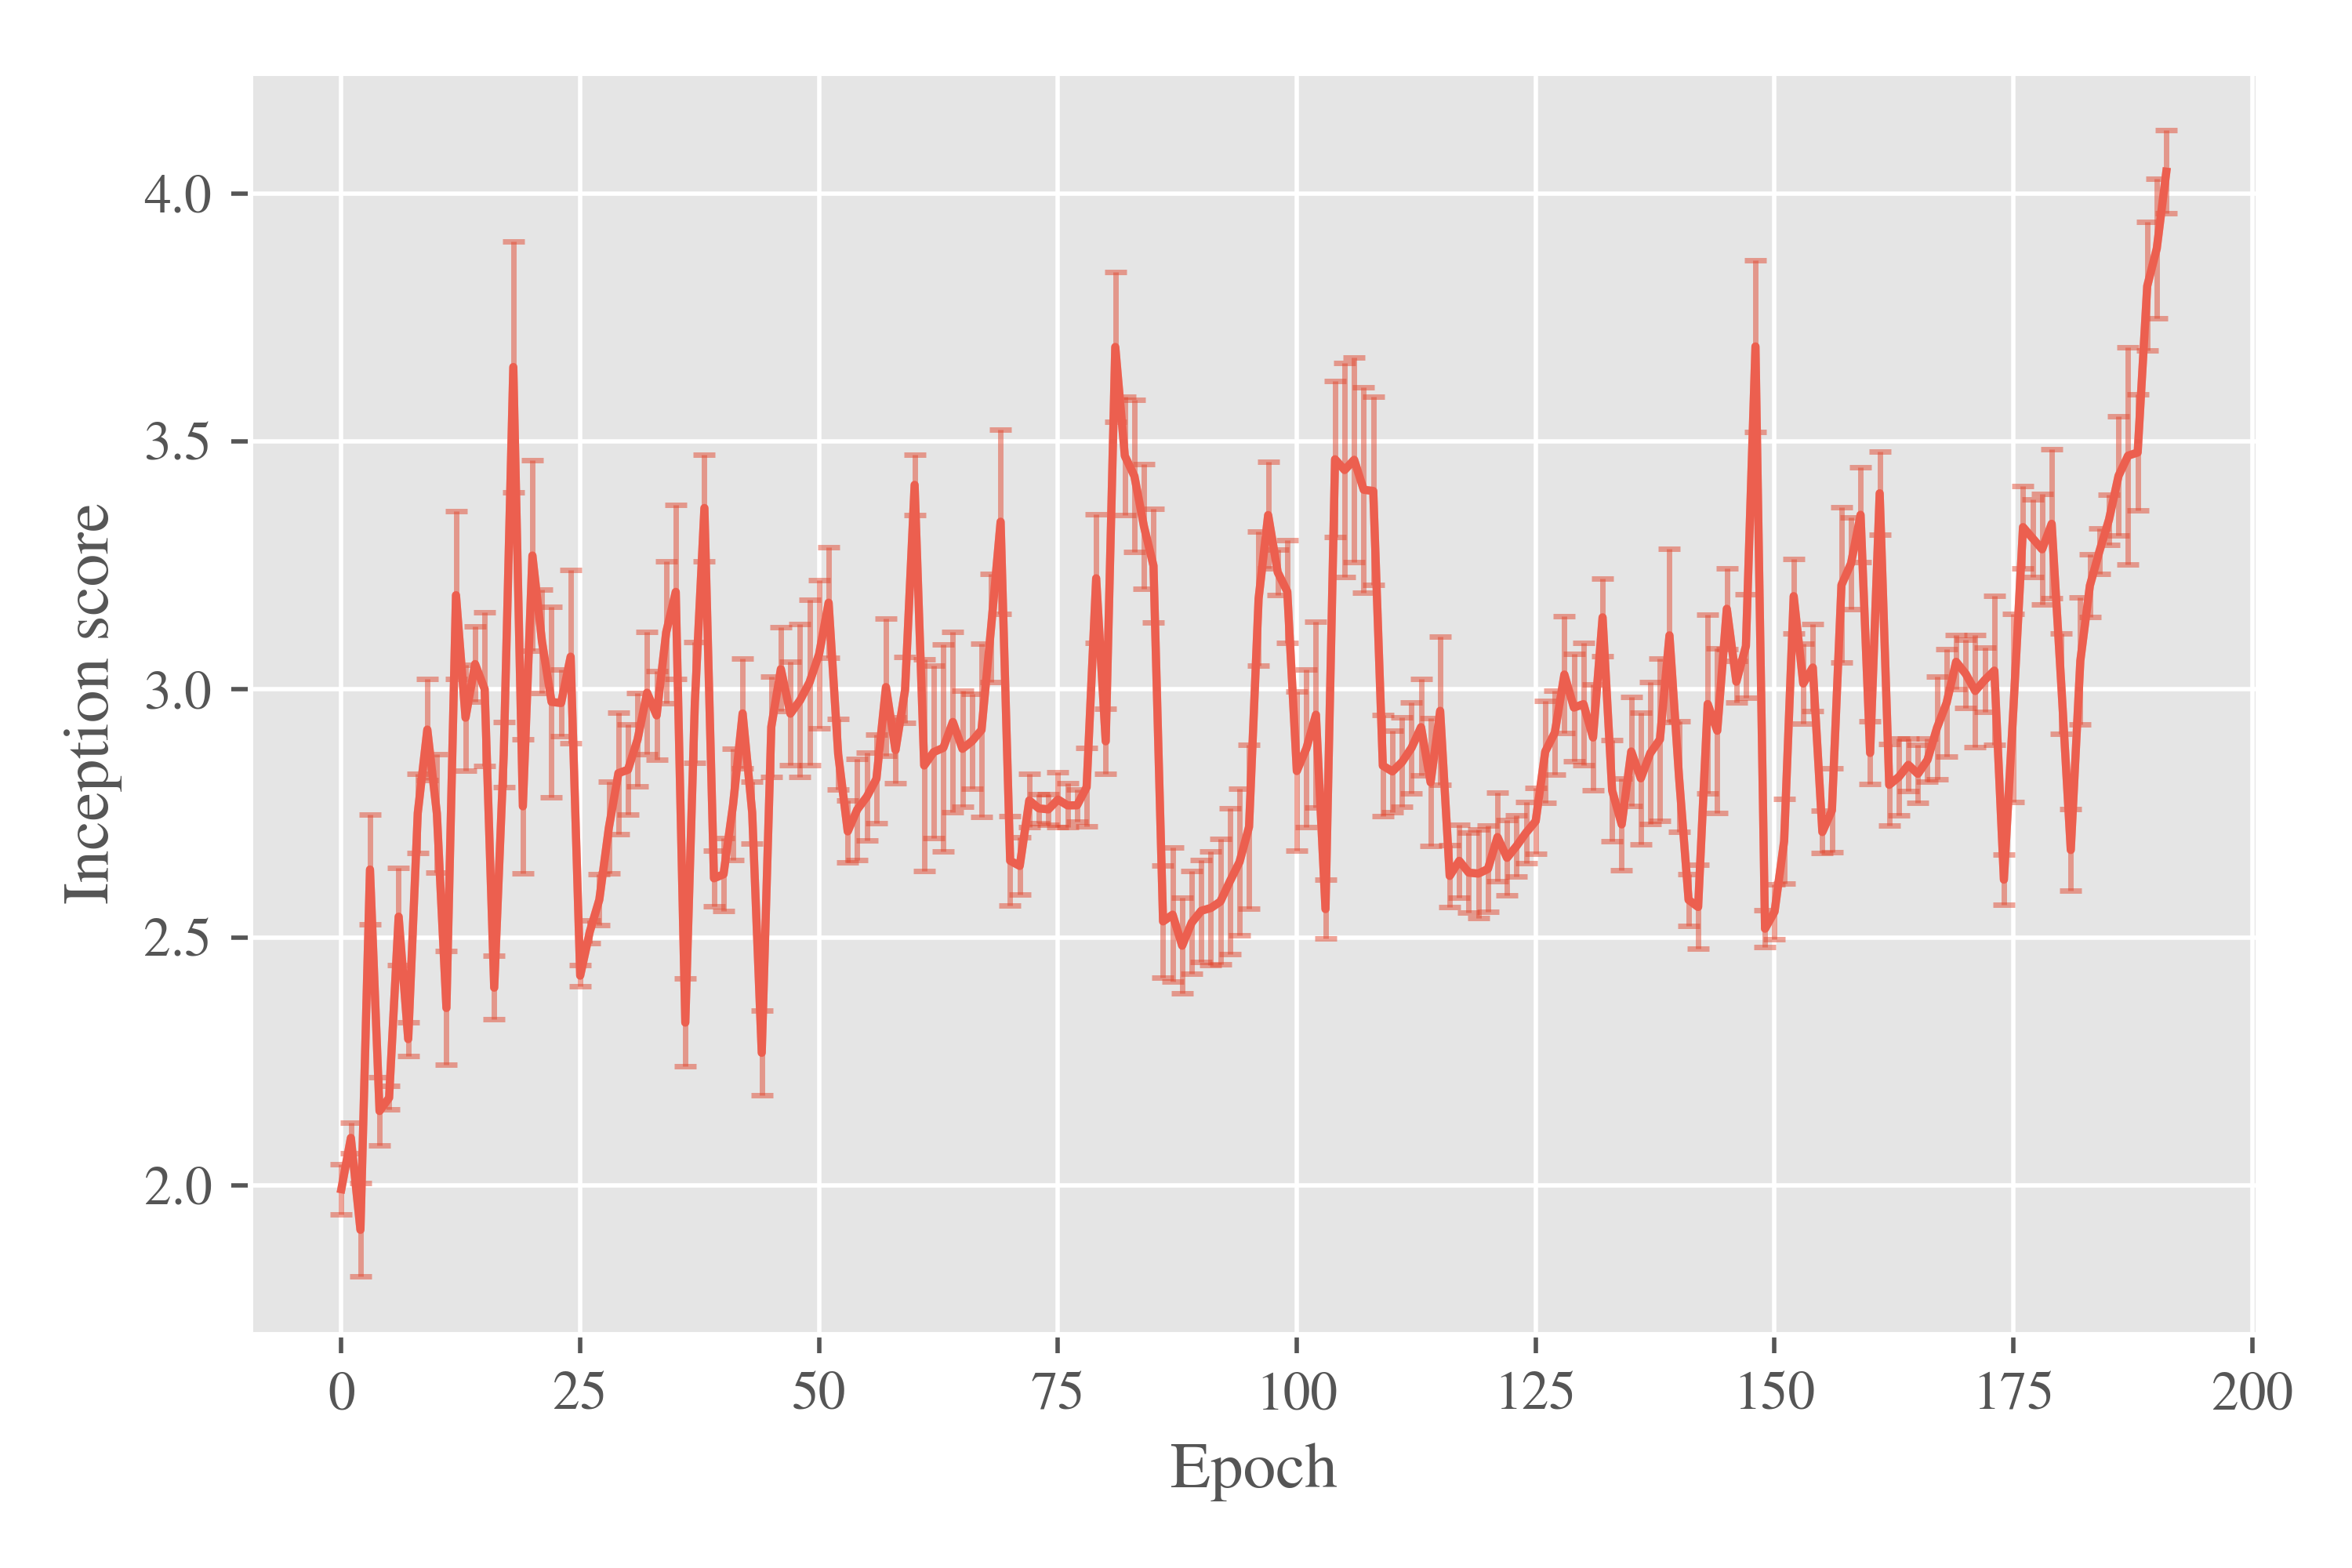
\includegraphics[width=\textwidth]{../code/results/figures/w-dcgan_cifar10_is.png}
		\caption{Inception score\\~}
		\label{fig:exp-w-dcgan-is}
    \end{subfigure}
    \begin{subfigure}[t]{0.49\textwidth}
        \centering
        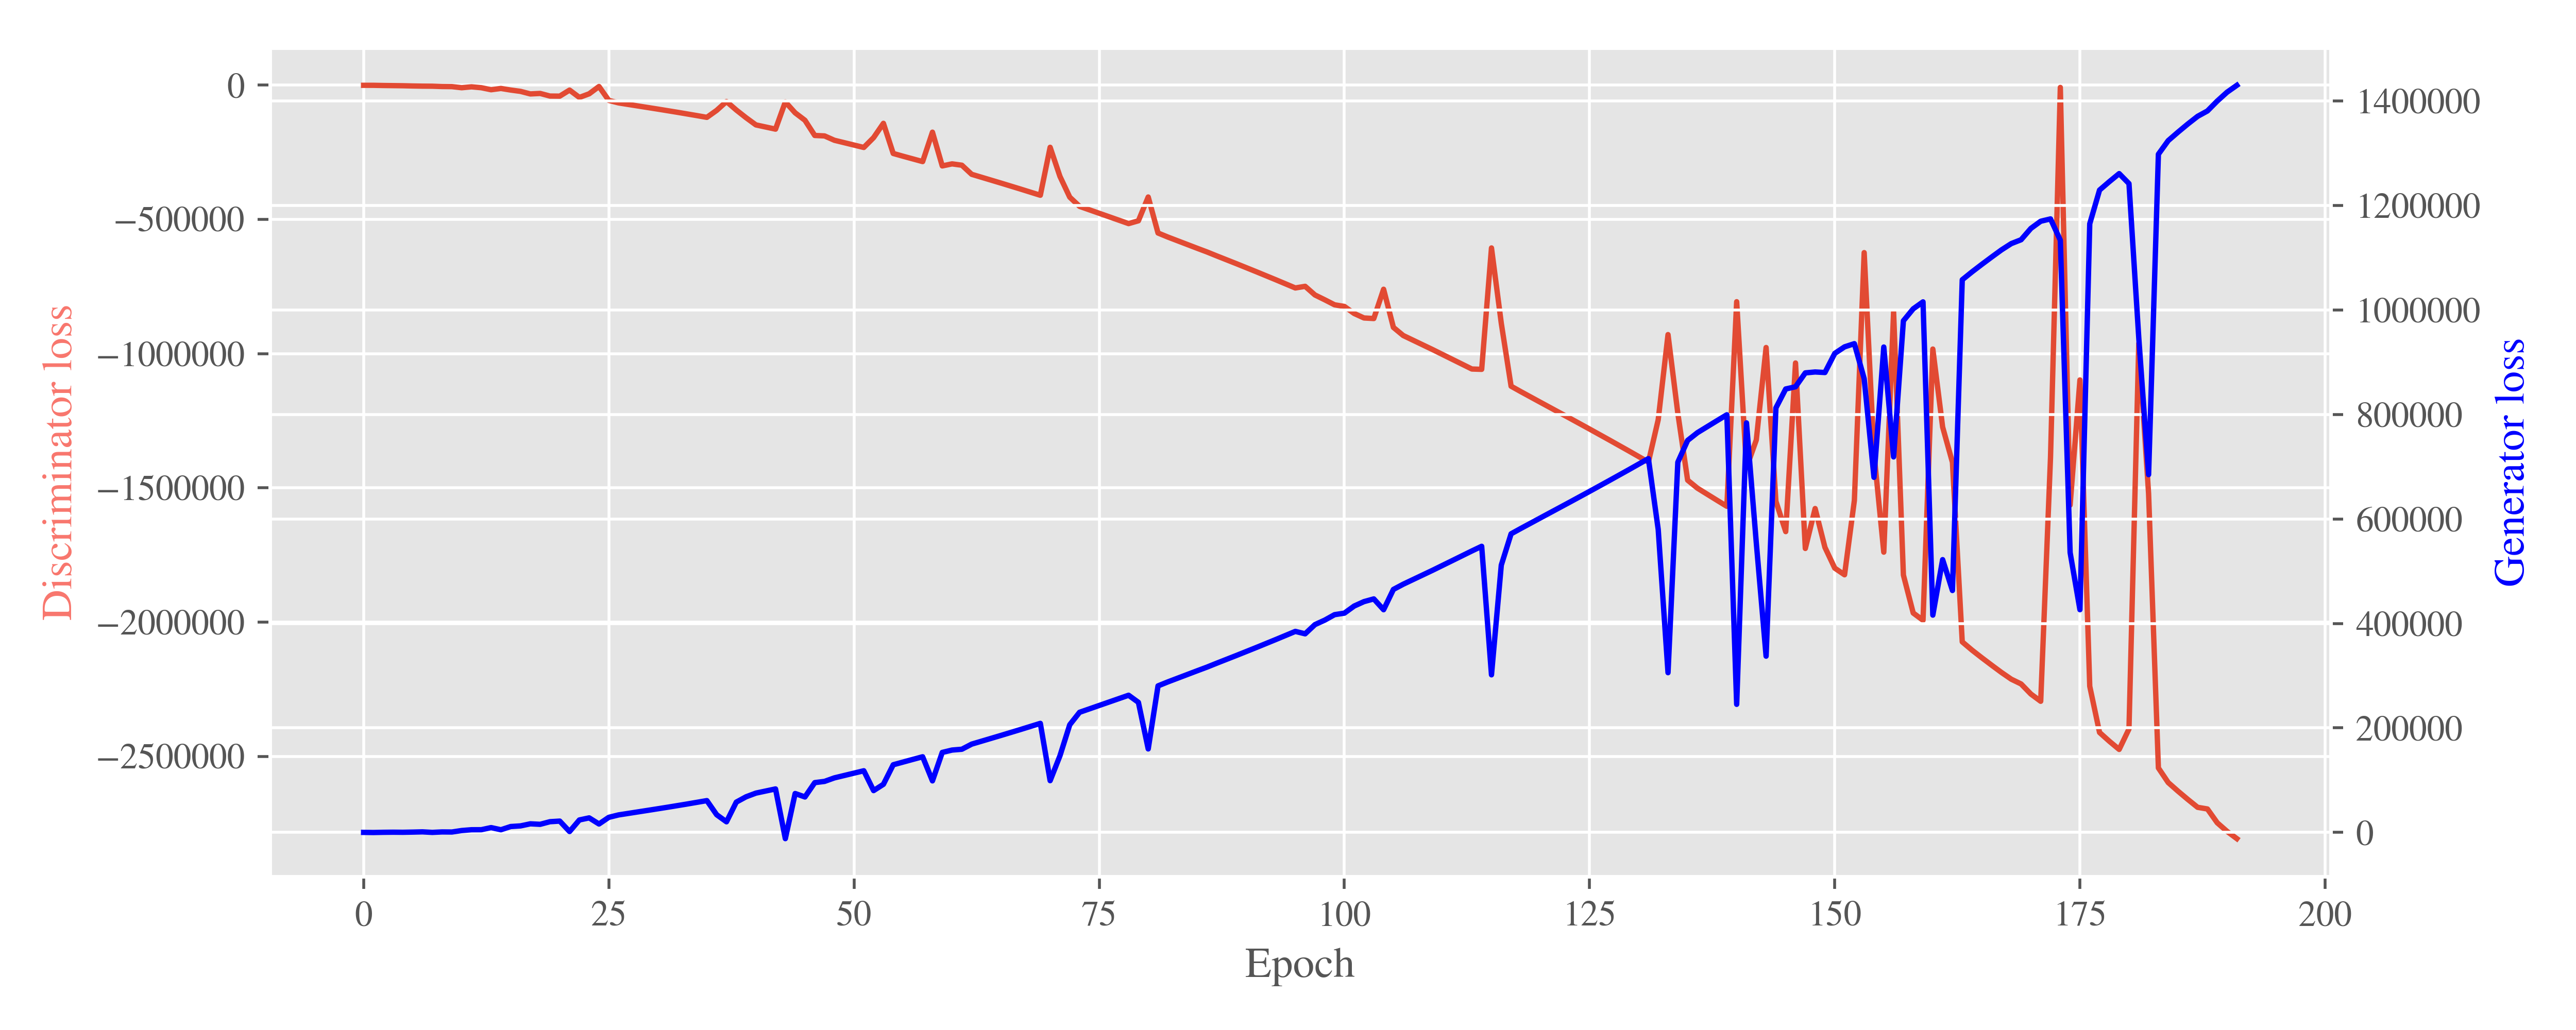
\includegraphics[width=\textwidth]{../code/results/figures/w-dcgan_cifar10_losses.png}
		\caption{Losses\\~}
		\label{fig:exp-w-dcgan-losses}
    \end{subfigure}
    \caption{W-DCGAN - training on CIFAR10 over 200 epochs.}
\end{figure}

%We observe that both losses are much smoother with spectral normalization. This is the desired result; the original intent of the paper on spectral normalization was to provide a solution to stabilize the training of GANs \cite{miyato2018spectral}. By visual inspection of the generated images we observe a significant reduce in mode collapse and a noticeable improvement of image quality. This did however not result in a significant Inception score improvement.